% Options for packages loaded elsewhere
\PassOptionsToPackage{unicode}{hyperref}
\PassOptionsToPackage{hyphens}{url}
%
\documentclass[
  english,
  man,floatsintext]{apa6}
\usepackage{amsmath,amssymb}
\usepackage{lmodern}
\usepackage{iftex}
\ifPDFTeX
  \usepackage[T1]{fontenc}
  \usepackage[utf8]{inputenc}
  \usepackage{textcomp} % provide euro and other symbols
\else % if luatex or xetex
  \usepackage{unicode-math}
  \defaultfontfeatures{Scale=MatchLowercase}
  \defaultfontfeatures[\rmfamily]{Ligatures=TeX,Scale=1}
\fi
% Use upquote if available, for straight quotes in verbatim environments
\IfFileExists{upquote.sty}{\usepackage{upquote}}{}
\IfFileExists{microtype.sty}{% use microtype if available
  \usepackage[]{microtype}
  \UseMicrotypeSet[protrusion]{basicmath} % disable protrusion for tt fonts
}{}
\makeatletter
\@ifundefined{KOMAClassName}{% if non-KOMA class
  \IfFileExists{parskip.sty}{%
    \usepackage{parskip}
  }{% else
    \setlength{\parindent}{0pt}
    \setlength{\parskip}{6pt plus 2pt minus 1pt}}
}{% if KOMA class
  \KOMAoptions{parskip=half}}
\makeatother
\usepackage{xcolor}
\IfFileExists{xurl.sty}{\usepackage{xurl}}{} % add URL line breaks if available
\IfFileExists{bookmark.sty}{\usepackage{bookmark}}{\usepackage{hyperref}}
\hypersetup{
  pdftitle={The role of cognateness in non-native spoken word recognition},
  pdfauthor={Gonzalo Garcia-Castro1, Serene Siow2, Nuria Sebastian-Galles1, \& Kim Plunkett2},
  pdflang={en-EN},
  pdfkeywords={cognate, word recognition, translation, non-native, spoken word recognition},
  hidelinks,
  pdfcreator={LaTeX via pandoc}}
\urlstyle{same} % disable monospaced font for URLs
\usepackage{graphicx}
\makeatletter
\def\maxwidth{\ifdim\Gin@nat@width>\linewidth\linewidth\else\Gin@nat@width\fi}
\def\maxheight{\ifdim\Gin@nat@height>\textheight\textheight\else\Gin@nat@height\fi}
\makeatother
% Scale images if necessary, so that they will not overflow the page
% margins by default, and it is still possible to overwrite the defaults
% using explicit options in \includegraphics[width, height, ...]{}
\setkeys{Gin}{width=\maxwidth,height=\maxheight,keepaspectratio}
% Set default figure placement to htbp
\makeatletter
\def\fps@figure{htbp}
\makeatother
\setlength{\emergencystretch}{3em} % prevent overfull lines
\providecommand{\tightlist}{%
  \setlength{\itemsep}{0pt}\setlength{\parskip}{0pt}}
\setcounter{secnumdepth}{-\maxdimen} % remove section numbering
% Make \paragraph and \subparagraph free-standing
\ifx\paragraph\undefined\else
  \let\oldparagraph\paragraph
  \renewcommand{\paragraph}[1]{\oldparagraph{#1}\mbox{}}
\fi
\ifx\subparagraph\undefined\else
  \let\oldsubparagraph\subparagraph
  \renewcommand{\subparagraph}[1]{\oldsubparagraph{#1}\mbox{}}
\fi
% Manuscript styling
\usepackage{upgreek}
\captionsetup{font=singlespacing,justification=justified}

% Table formatting
\usepackage{longtable}
\usepackage{lscape}
% \usepackage[counterclockwise]{rotating}   % Landscape page setup for large tables
\usepackage{multirow}		% Table styling
\usepackage{tabularx}		% Control Column width
\usepackage[flushleft]{threeparttable}	% Allows for three part tables with a specified notes section
\usepackage{threeparttablex}            % Lets threeparttable work with longtable

% Create new environments so endfloat can handle them
% \newenvironment{ltable}
%   {\begin{landscape}\centering\begin{threeparttable}}
%   {\end{threeparttable}\end{landscape}}
\newenvironment{lltable}{\begin{landscape}\centering\begin{ThreePartTable}}{\end{ThreePartTable}\end{landscape}}

% Enables adjusting longtable caption width to table width
% Solution found at http://golatex.de/longtable-mit-caption-so-breit-wie-die-tabelle-t15767.html
\makeatletter
\newcommand\LastLTentrywidth{1em}
\newlength\longtablewidth
\setlength{\longtablewidth}{1in}
\newcommand{\getlongtablewidth}{\begingroup \ifcsname LT@\roman{LT@tables}\endcsname \global\longtablewidth=0pt \renewcommand{\LT@entry}[2]{\global\advance\longtablewidth by ##2\relax\gdef\LastLTentrywidth{##2}}\@nameuse{LT@\roman{LT@tables}} \fi \endgroup}

% \setlength{\parindent}{0.5in}
% \setlength{\parskip}{0pt plus 0pt minus 0pt}

% \usepackage{etoolbox}
\makeatletter
\patchcmd{\HyOrg@maketitle}
  {\section{\normalfont\normalsize\abstractname}}
  {\section*{\normalfont\normalsize\abstractname}}
  {}{\typeout{Failed to patch abstract.}}
\patchcmd{\HyOrg@maketitle}
  {\section{\protect\normalfont{\@title}}}
  {\section*{\protect\normalfont{\@title}}}
  {}{\typeout{Failed to patch title.}}
\makeatother
\shorttitle{Cognateness and non-native word recognition}
\keywords{cognate, word recognition, translation, non-native, spoken word recognition\newline\indent Word count: X}
\usepackage{lineno}

\linenumbers
\usepackage{csquotes}
\ifXeTeX
  % Load polyglossia as late as possible: uses bidi with RTL langages (e.g. Hebrew, Arabic)
  \usepackage{polyglossia}
  \setmainlanguage[]{english}
\else
  \usepackage[main=english]{babel}
% get rid of language-specific shorthands (see #6817):
\let\LanguageShortHands\languageshorthands
\def\languageshorthands#1{}
\fi
\ifLuaTeX
  \usepackage{selnolig}  % disable illegal ligatures
\fi
\newlength{\cslhangindent}
\setlength{\cslhangindent}{1.5em}
\newlength{\csllabelwidth}
\setlength{\csllabelwidth}{3em}
\newenvironment{CSLReferences}[2] % #1 hanging-ident, #2 entry spacing
 {% don't indent paragraphs
  \setlength{\parindent}{0pt}
  % turn on hanging indent if param 1 is 1
  \ifodd #1 \everypar{\setlength{\hangindent}{\cslhangindent}}\ignorespaces\fi
  % set entry spacing
  \ifnum #2 > 0
  \setlength{\parskip}{#2\baselineskip}
  \fi
 }%
 {}
\usepackage{calc}
\newcommand{\CSLBlock}[1]{#1\hfill\break}
\newcommand{\CSLLeftMargin}[1]{\parbox[t]{\csllabelwidth}{#1}}
\newcommand{\CSLRightInline}[1]{\parbox[t]{\linewidth - \csllabelwidth}{#1}\break}
\newcommand{\CSLIndent}[1]{\hspace{\cslhangindent}#1}

\title{The role of cognateness in non-native spoken word recognition}
\author{Gonzalo Garcia-Castro\textsuperscript{1}, Serene Siow\textsuperscript{2}, Nuria Sebastian-Galles\textsuperscript{1}, \& Kim Plunkett\textsuperscript{2}}
\date{}


\authornote{

GG and SS contributed equally and share first authorship.

The authors made the following contributions. Gonzalo Garcia-Castro: Conceptualization, Data analysis, Writing - Original Draft Preparation, Writing - Review \& Editing; Serene Siow: Conceptualization, Writing - Review \& Editing; Nuria Sebastian-Galles: Conceptualization, Writing - Review \& Editing; Kim Plunkett: Conceptualization, Writing - Review \& Editing.

Correspondence concerning this article should be addressed to Gonzalo Garcia-Castro, Ramon Trial Fargas, 25-27, 08005 Barcelona. E-mail: \href{mailto:gonzalo.garciadecastro@upf.edu}{\nolinkurl{gonzalo.garciadecastro@upf.edu}}

}

\affiliation{\vspace{0.5cm}\textsuperscript{1} Center for Brain and Cognition, Universitat Pompeu Fabra\\\textsuperscript{2} Department of Experimental Psychology, University of Oxford}

\abstract{
There is compelling evidence that bilinguals access their lexicon in a language non-selective way. For example, bilinguals produce and translate cognates (words whose translation in the other language is form-similar) faster than non-cognates, suggesting that the phonology of both languages interact during word production and comprehension (Costa et al., 2000; Christoffels et al., 2006). Previous literature on this effect has often relied on measures of overall form-similarity to categorise words into cognates andnon-cognates, such as the Levenshtein distance. These measures partially ignore potential sources of variability during lexical access like vowel vs.~consonant overlap, overlap in stressed syllables, onset overlap or the distance in features between both translations. In this study, we explored the impact of some of these variables on non-native word translation task: Spanish and English participants listened to non-native words (Catalan or Spanish) and were prompted to type their translation in their native language. Critically, participants where unfamiliar with the testing language, ensuring that they were not able to translate words based on previous knowledge on their meaning, leaving phonological information as the only cue participants were able to exploit to translate words to their native language correctly. We analysed the probability of correct translations, adjusting for the amount of vowel overlap, consonant overlap, overlap at stress position, overlap at onset, and distance in features between replaced phonemes, including the average frequency of phonological neighbours of the target words are a covariate.
}



\begin{document}
\maketitle

\hypertarget{introduction}{%
\section{Introduction}\label{introduction}}

\hypertarget{native-speech-processing-is-effortless}{%
\subsection{Native speech processing is effortless}\label{native-speech-processing-is-effortless}}

Humans are able to recognise spoken words without much effort, even in adverse conditions such as compressed speech (De Haan, 1982) or the loss of segmental information (Warren, 1970). But even in the most ideal of the situations, the processes engaged in word recognition do not occur without uncertainty. The speech input activates multiple candidate lexical representations based on their similarity with the signal, and for word recognition to take place, one of the candidates must be selected. There is extensive literature about how the number of candidates, their frequency, and their phonological and semantic similarity with the target word impacts the dynamics of word recognition. But less is known about how these factors affect the recognition of words in a non-native language.

\hypertarget{non-antive-speech-processing-is-costly}{%
\subsection{Non-antive speech processing is costly}\label{non-antive-speech-processing-is-costly}}

Listening to speech in a non-native language is more costly than doing so in the native language, even if one is proficient in such language. The source of this increased cognitive effort is likely to originate at multiple levels. Some examples: (1) some sounds in the speech signal do not correspond to any phoneme in the native language, (2) segmenting the speech signal relies on previous familiarity with word forms or with the statistical regularities of the language: (3) word order might be different in both languages (e.g., subject-object-verb vs.~subject-verb-object.). The listener, however, is rarely completely naïve to the language they are listening to. All languages share, to some extent, similarities, frequently due to their typological closeness. These similarities which can be exploited by non-native listeners.

\hypertarget{cognateness-aids-non-native-speech-processing}{%
\subsection{Cognateness aids non-native speech processing}\label{cognateness-aids-non-native-speech-processing}}

One of such commonalities occurs at the lexical level, in the for of cognateness. Cognates are cross-language synonyms whose form (e.g., phonology, orthography, signature) is similar. The cause of this similarity is frequently attributed to a shared etymological origin. Romance languages like Spanish, Italian, French or Catalan, share many cognates (Schepens, Dijkstra, \& Grootjen, 2012). For example, this is the case of \emph{puerta} and \emph{porta} (\emph{door} in Spanish and Catalan, respectively)\footnote{Some form-similar cross-language synonyms are technically not cognates. For example, \emph{sun} and \emph{sol} (in Spanish), share their phonological onset, but their etymology points to different origins. We will use the word \emph{cognateness} to include all form-similar cross-language synonyms for simplicity. It is highly implausible that etymology plays a direct role on language perception if it is not via form-similarity, since it is not necessary for participants in psycholinguistic experiments to be aware of the etymology of the words they encounter in the tasks to be subject to the effect of form-similarity.}.

\hypertarget{the-cognate-advantage-in-comprehension-production-and-learning}{%
\subsection{The cognate advantage in comprehension, production, and learning}\label{the-cognate-advantage-in-comprehension-production-and-learning}}

Cognates play a major role in virtually all models of bilingual lexical processing because they provide evidence that bilinguals access their lexicon in a language non-selective way: during word production and comprehension, both lexical representations are activated, and the form similarity between both impacts participants' performance in naming or lexical decision tasks (e.g., Costa, Caramazza, \& Sebastian-Galles, 2000; Thierry \& Wu, 2007). For instance, in their seminal study, Costa et al. (2000) asked Spanish-Catalan bilinguals to name pictures in Spanish. Unbeknownst to participants, half of the pictures' associated labels were cognates in Spanish and Catalan (e.g., \emph{puerta}-\emph{porta}) while the other half were non-cognates (e.g., \emph{mesa}-\emph{taula}). Surprisingly, participants named cognate pictures faster than non-cognate pictures, while Spanish monolinguals did not show this effect. This suggested that bilinguals activated picture's word representations in both languages, and that the phonological overlap between both labels facilitated the naming process.

There is also evidence that cognates are learnt more easily in L2 than non-cognates. For instance, De Groot and Keijzer (2000) presented 40 Dutch natives 60 pairs of translation equivalents. In each learning trial, two words were presented in a screen side-by-side: one in Dutch and one pseudoword. Pseudowords were generated in such way that were easily pronounceable and were phonotactically legal in Dutch. Word pairs varied in their form-similarity (number of shared letters, 40-70\%). Participants were tested twice in the same task with one week of difference. Participants' performance was better for cognates across both testing sessions, suggesting that cognates were learnt and retained more easily than non-cognates. Converging evidence was provided by Lotto and De Groot (1998) in Dutch natives learning Italian words: cognates were learnt more easily than non-cognates.

\hypertarget{the-cognate-advantage-in-translation-the-rmh-model}{%
\subsubsection{The cognate advantage in translation: the RMH model}\label{the-cognate-advantage-in-translation-the-rmh-model}}

Cognates are not only learnt faster than non-cognates, but translated faster too. The mechanisms behind this effect, though, are still unclear. Early accounts of bilingual lexical access suggested that low-proficiency learners first established links between newly learnt words in L2 and their meanings through their L1 translation equivalents (Potter, So, Von Eckardt, \& Feldman, 1984). As learners become more proficient, the connection between L2 representations and their meaning grows stronger, and L2 word processing becomes less reliant on the mediation of L1 representations. The Revised Hierarchical Model {[}RHM; Kroll and Stewart (1994){]} captured this assumption and predicted that translating words from L1 to L2 (forward translation) should take longer than translating from L2 to L1 (backward translation). The rationale behind this prediction is that backward translation relies more strongly on direct word-word links between L1 and L2 representations, while forward translation would rely more strongly on the mediation between the concept and the two word forms. One of the consequences of this prediction is that backward translation should be more sensitive to the form similarity between the L1 and the L2 representations: cognate words should be retrieved faster than non-cognate words during backward translation.

To test these predictions, Degroot, Dannenburg, and Vanhell (1994) and Groot (1992) asked 52 Dutch natives with high (yet non-native) English proficiency to translate words from either Dutch to English (forward translation, L1 to L2) or from English to Dutch (backward translation, L2 to L1). In each trial, participants were presented visually with a word in English or Dutch, and were asked to speak out loud its translation in the other language as soon as possible. The authors reported three main findings: (1) translation times and accuracy were roughly equivalent in across both forward and backward conditions (although slightly faster in the former), (2) semantic variables, such as imageability, were positively associated with participants' performance more strongly in the forward translation conditional, although the effect size was small, (3) cognates were translated equally fast in both conditions, but non-cognates were translated faster during backward translation than during forward translation, and (4) when translating cognates participants' performance across both conditions was less sensitive to semantic variables than when translating non-cognates. These results prompted the authors to reject a hard version Kroll and Stewart (1994)'s account, and suggested that both conceptually mediated and direct translation routes are active during translation, but backward translation relies more strongly on direct links between L1 and L2 representations, which makes it more sensitive to cognateness than forward translation. When the authors tested a group of bilinguals with higher proficiency in English, their results pointed in the same direction. Subsequent studies did not find differences in participant's performance during forward and backward translation, or even found better performances in forward translation (Christoffels, De Groot, \& Kroll, 2006; Christoffels, Ganushchak, \& Koester, 2013), contrary to the predictions of the RHM.

\hypertarget{the-impact-of-neighbourhoods-lexical-processing-the-nam-and-the-biabia-models}{%
\subsection{The impact of neighbourhoods lexical processing: the NAM and the BIA/BIA+ models}\label{the-impact-of-neighbourhoods-lexical-processing-the-nam-and-the-biabia-models}}

The idealised lexicon considered by the models described above only considers word-word connections between translation equivalents. More recent studies have highlighted the role of the rich network of connections that given word establishes with other phonologically or conceptually related words. This notion was first introduced in monolingual research by Collins and Loftus (1975) in their theory of semantic processing, and later Luce and Pisoni (1998) formalised this dimension in their Neighbourhood Activation Model (NAM). In this model, lexical selection is mediated not only by the lexical frequency of the target word, and the number of activated candidates, but also by the frequency of the candidates. Luce and Pisoni (1998) designed a lexical decision task in which English native participants listened to a word across several conditions of noise-to-signal ratio. The authors then used a computerised lexicon to calculate the number of phonological neighbours around each of the presented words, based on phonetic similarity matrices, and the average lexical frequency of such neighbourhoods. Participants answered more faster and more accurately to high frequency words. Words from high density neighbourhoods were responded to more accurately, but more slowly. The average lexical frequency of the neighbourhood was associated to a decrease in accuracy. Low frequency words were responded to more accurately in low density neighbours than in high density neighbours. The authors concluded that, although both word lexical frequency and neighbourhood density can, in principle, facilitate spoken word recognition, this effect was modulated by the frequency of the neighbourhood: when phonological neighbours are more frequent, lexical selection is hindered (Goldinger, Luce, \& Pisoni, 1989; Luce, Pisoni, \& Goldinger, 1990).

The fact that phonological neighbourhoods and their structure impacts lexical processing poses an important question for bilingualism research. Are word representations in one language part of phonological or orthographic neighbours in the other language? Van Heuven, Dijkstra, and Grainger (1998) addressed this issue in an experimental series and proposed the Bilingual Interactive Activation (BIA, later revised and relabelled as BIA+). In line with connectionist accounts of lexical processing this model advocated for lexical representations to establish both excitatory and inhibitory connections with other representations from the same of the other language (McClelland \& Rumelhart, 1981), forming an integrated lexicon for both languages. Van Heuven et al. (1998) tested Dutch-English bilinguals in a progressive demasking task (in each trial a words in presented in increasingly longer time windows interrupted by a checkerboard until the participant presses a button to type the word in a keyboard) or a lexical decision task (words a visually presented and the participant must decide as quickly as possible whether its a word in the target language or a non-word). The authors manipulated by size of the orthographic neighbourhood size of the words presented in its language (target language) or in the other language (non-target language). Interestingly, the authors reported participants' performance to be affected by the neighbourhood size of the presented word in the non-target language across both tasks. Specifically, participants took longer to respond to words with high neighbourhood density in the non-target language, even when participants completed the task in the target language exclusively (e.g., were presented with Dutch words exclusively). Monolinguals, on the other hand, were only affected by neighbourhood size in the target language. This provided evidence of cross-language interference between the word representation in the non-target language and the those in the target language.

\hypertarget{is-the-lexical-route-necessary-for-translation-the-multilink-model}{%
\subsection{Is the lexical route necessary for translation?: The Multilink model}\label{is-the-lexical-route-necessary-for-translation-the-multilink-model}}

More recently, Dijkstra et al. (2019) implemented a localist-connectionist model, Multilink, that integrates and formalises previous claims and predictions on how an interactive account of bilingual lexical access impacts word recognition, production, and more relevant to the aims of the present study, translation. This model assumes (1) an integrated lexicon in which word representations from the two languages establish connections as words from the same language do; (2) during backward translation, the presented word in L2 can activate form-similar words in L1 that compete with the target word in L1; (3) contrary to the RHM model's assumption that translation equivalents are linked by excitatory connections (e.g., translation can be done via word-word connections), Dijkstra et al. (2019) suggest that such connections would spread activation though irrelevant words in the target language and therefore initially assumed that translation equivalents are exclusively connect throught their shared concept; (4) the strength of the association between L2 representations and their concept is a function of the language user's proficiceny in L2. Multilink considers the particular case of Dutch-English bilinguals to generated simulations and test them against experimental data. The authors simulated data from Multilink to mirror Christoffels et al. (2006) translation elicitation task, and reported a remarkable correlation between Multilink's simulations and participant's data, with forward translation being faster than backward translation, contrary to the RHM model predictions. More relevant to the present study is the fact that the model also generated data suggesting that cognates are translated faster than non-cognates, in line with previous literature on the cognate advantage during translation. Overall, evidence from this model provides evidence for an integrated bilingual lexicon and for a facilitatory effect of cross-language similarity during translation. One of the main conclusions of Dijkstra et al. (2019) study is that word-word connections are not necessary for translation, as suggested by Kroll and Stewart (1994): Multilink did not include such connections and still fitted experimental data. However, as they note, both their simulations and the data collected by Christoffels et al. (2006) corresponded to high-proficiency bilinguals. In the case of the model simulations, vocabulary sizes were balanced in both languages and word-concept connections were equally strong for each member of the translation pairs in both languages. This scenario is actually contemplated by the Kroll and Stewart (1994)'s RHM model. What Dijkstra et al. (2019) did not test, is the fit of Mutilink's predictions for low-proficiency, unbalanced bilinguals, whose vocabulary sizes are smaller or their word-concept connections are weaker in L2 than in L1. It is under this set of assumptions that the RHM model predicts participants to rely strongly on word-word connections to be able to translation words, especially from L2 to L1. This prediction, however, is untested in the Multilink model.

\hypertarget{the-present-study}{%
\subsection{The present study}\label{the-present-study}}

In this study, we explored the plausibility of the lexical route in backward translation by testing monolingual participants. Monolinguals can be considered a particular (extreme) case of unbalanced bilingualism, in which which participants' vocabulary size in L2 is null, and word-concept connections are absent (i.e., set to zero in formal terms). In this scenario, participants can only rely on the similarity between the L2 form (presented as stimulus) and the L1 form (the target word). In other words, these participants can only use the lexical route to suceeed in the translation task. If participants are able to translate words in L2, even with no knowledge of the language it belongs to, based on their form-similarity with the target word, this would sugges that the lexical route is in place for low-proficiency bilinguals. If participants are not able to translation words from L2 to L1 regardless of their form-similarity, this would suggest that low-proficiency bilinguals rely entirely on word-concept connections for backward translation.

\hypertarget{methods}{%
\section{Methods}\label{methods}}

\hypertarget{participants}{%
\subsection{Participants}\label{participants}}

Data collection took place from June 04th, 2020 to June 28th, 2020. We collected data from 104 participants (\emph{Mean} = 21.79 years, \emph{SD} = 2.43, Range = 18-33). 72 participants were British English native speakers living in United Kingdom (46 female), and 32 participants were Spanish native speakers living in Spain (27 female). Participants in UK were recruited via Prolific (5£ compensation) and SONA (compensation in academic credits). Participants in Spain were contacted via announcements in Faculties, and were compensated 5€ or an Amazon voucher for the same value. Participants gave informed consent before providing any data and the study was conducted in accordance with ethical standards of the Declaration of Helsinki and the protocol was approved by the local ethical committee (XXXXXXXXXXXX). Participants were asked to complete the experiment using a laptop in a quiet place with good internet connection. We excluded data from participants that a) self-rated their oral and/or written skills in a second or third language as higher than 4 in a 5-point scale (\emph{n} = 1), b) were diagnosed with a language (\emph{n} = 2) , or c) did not contribute more than 80\% of valid trials (\emph{n} = 9).

\hypertarget{procedure}{%
\subsection{Procedure}\label{procedure}}

The experiment was implemented online using Psychopy/Pavlovia (Peirce et al., 2019). Participants accessed the study from a link provided by Prolific or SONA and completed the experiment from an internet browser (Chrome or Mozilla). After giving their consent for participating, participants answered a series of questions about their demographic status, their language background, and the set up they were using for completing the study. Then, participants completed the experimental task. Participants were informed that they would listen to a series of pre-recorded words in Catalan or Spanish (English participants) or only Catalan (Spanish participants). They were instructed to listen to each word, guess its meaning in English (English participants) or Spanish (Spanish participants), and type their answer as soon as possible. English participants were randomly assigned to the list of Catalan or Spanish trials. Participants in the Catalan list were presented with 86 trials, and participants in the Spanish list were presented with 103 trials.

\begin{figure}
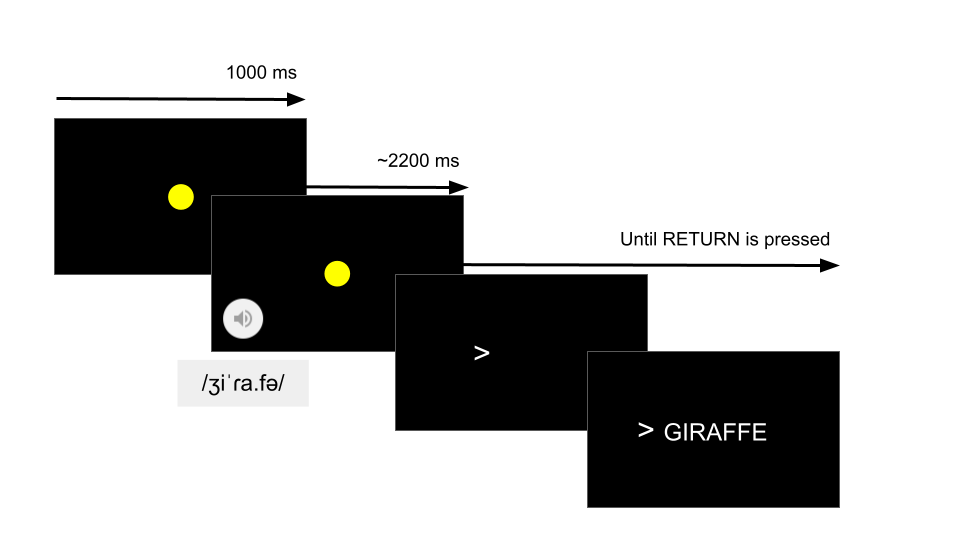
\includegraphics[width=0.8\linewidth]{C:/Users/u155880/Documents/translation-elicitation/Figures/design} \caption{ }\label{fig:procedurefigure}
\end{figure}

Each trial started with a yellow fixation point presented during one second on the centre of the screen over a black background. After one second, the audio started playing while the dot remained being displayed until the audio ended. Upon the offset of the fixation point and audio, participants were prompted to write their answer by a ``\textgreater{}'' symbol. Typed letters were displayed in the screen in real time to provide visual feed-back to participants. Participants were allowed to correct their answer. Then, participants pressed the RETURN key to start and new trial. We excluded trials where participants did not type an existing word in the correspondent language, or did not type anything at all. Trials where the response was mistyped by only one character were counted as correct, as long as the respond did not correspond to a distinct word. Participants contributed a total of 8077 valid trials (5235 in Catalan, 2842 in Spanish). The task took approximately 15 minutes to be completed.

\hypertarget{stimuli}{%
\subsection{Stimuli}\label{stimuli}}

We arranged two lists of words: one in Catalan (to be presented to English and Spanish natives) and one in Spanish (to be presented to English natives only). Words in the Catalan list (listened to by participants) were 5.01 phonemes long on average (\emph{SD} = 1.48, Range = 2-8). Their translations to English (typed by participants in the keyboard) were 5.14 characters long on average (\emph{SD} = 1.57, Range = 3-9), and their translations to Spanish were 5.44 characters long on average (\emph{SD} = 1.56, Range = 3-9). Words in the Spanish list were 5.50 phonemes long on average (\emph{SD} = 1.46, Range = 3-9). Their translations to English were 5.27 characters long on average (\emph{SD} = 1.75, Range = 3-12).

We extracted the lexical frequencies from SUBTLEX-UK for English words (Van Heuven, Mandera, Keuleers, \& Brysbaert, 2014), SUBTLEX-ESP for Spanish words (Cuetos, Glez-Nosti, Barbon, \& Brysbaert, 2011), and SUBTLEX-CAT for Catalan words (Boada, Guasch, Haro, Demestre, \& Ferré, 2020). We extracted or transformed scores as/into Zipf scores (Van Heuven et al., 2014) to so correct their logarithmic distribution, limiting their range roughly between 0 to 7, allowing an easier interpretation of further analyses (Van Heuven et al., 2014).

We retrieved PTHN scores from the CLEARPOND database (Marian, Bartolotti, Chabal, \& Shook, 2012). PTHN scores indicate the number of phonological neighbours of the target word with higher lexical frequency, as indicated by its score in the corresponding SUBTLEX database. CLEARPOND defines a phonological neighbour as a word whose phonological transcription in International Phonetic Alphabet (IPA) format (generated from eSPEAK, \url{http://espeak.sourceforge.net/}) differs from that of the target word in only one addition, deletion, or substitution. PTHN scores in CLEARPOND measure have been calculated using corpora of similar size across language, allowing reliable cross-language comparisons.

Finally, we measured the phonological similarity between translation pairs by computing the Levenshtein similarity between their IPA translations using the \texttt{stringsim} function of the stringdist R package (van der Loo, 2014). This function computes the inverse of the Levenshtein distance between two character strings as a proportion. First, it computes the edit distance between two character strings (in this case, phoneme symbols) by counting the number of additions, deletions, and substitutions necessary to make both strings identical (Levenshtein \& others, 1966). This measure is then divided by the maximum distance (according to the length of the longest string) and then subtracted from 1. The result is a score that ranges from 0 to 1, where 0 indicates no similarity between the two strings and one indicates that both strings are identical. We computed this similarity measure (Levenshtein, from now on) for every translation pair in our stimuli lists. Table 1 summarises the lexical frequency, phonological neighbourhood density and phonological overlap of the words included in the Catalan and the Spanish lists.

Participants listened to one audio file in each trial. This audio file corresponded to a word in Catalan (for Spanish speakers, and for English participants allocated in the Catalan condition) or Spanish (for English speakers allocated in the Spanish condition). The audio files were the same ones used in child experiments conducted in the Laboratori de Recerca en Infància of Universitat Pompeu Fabra (Barcelona, Spain). These audio files were recorded by a proficient Catalan-Spanish female bilingual from the Metropolitan Area of Barcelona in a child-directed manner. Catalan and Spanish words were recorded at 44,100 Hz in separate files in the same session, and then de-noised using Audacity and normalised at peak intensity using Praat (Broersma \& Weenink, 2021). The average duration of the audios was 1.20 (\emph{SD} = 0.18, Range = 0.78-1.58). The average duration of the Catalan audios was 1.23 seconds (\emph{SD} = 0.19, Range = 0.80-1.58), and the average duration of the Spanish audios was 1.16 seconds (\emph{SD} = 0.15, Range = 0.78-1.53).

\captionsetup[table]{labelformat=empty,skip=1pt}
\begin{longtable}{lrrrrrrrr}
\toprule
 & \multicolumn{2}{c}{\textbf{Freq./million}} & \multicolumn{2}{c}{\textbf{Freq. (Zipf)}} & \multicolumn{2}{c}{\emph{\textbf{PTHN}}} & \multicolumn{2}{c}{\textbf{Levenshtein}} \\ 
 \cmidrule(lr){2-3} \cmidrule(lr){4-5} \cmidrule(lr){6-7} \cmidrule(lr){8-9}
 & Mean & \emph{SD} & Mean & \emph{SD} & Mean & \emph{SD} & Mean & \emph{SD} \\ 
\midrule
ENG-CAT & $46.80$ & $77.23$ & $4.31$ & $0.59$ & $3.26$ & $3.74$ & $0.16$ & $0.19$ \\ 
ENG-SPA & $43.91$ & $67.53$ & $4.32$ & $0.56$ & $3.52$ & $4.10$ & $0.13$ & $0.17$ \\ 
SPA-CAT & $53.32$ & $156.19$ & $4.23$ & $0.62$ & $1.62$ & $2.62$ & $0.37$ & $0.25$ \\ 
 \bottomrule
\end{longtable}

\hypertarget{data-analysis}{%
\subsection{Data analysis}\label{data-analysis}}

We modelled the probability of participants guessing the correct translation of each input word using a generalised multilevel Bayesian regression model with a Bernoulli logit link distribution. We first fitted a base model (Model 0) that only included the lexical frequency (\texttt{frequency}) of the target word as a fixed effect, with a random intercept per participant. Second, we extended the model to include \texttt{pthn} as a fixed effect, with a random slope by participant (Model 1). Third, we added the fixed effect \texttt{consonant\_ratio} and the \texttt{pthn:consonant\_ratio}, and random slopes for both effects by participant (Model 2). Third, we added the fixed effect \texttt{vowel\_ratio} and the \texttt{pthn:vowel\_ratio}, and random slopes for both effects by participant (Model 3). Finally, we fit a model that included the two-way interactions \texttt{pthn:consonant\_ratio} and \texttt{pthn:vowel\_ratio}, an their random slopes by participant (Model 4). All predictor variables were standardised (transformed in standard deviations from the mean) before entering the model. Model 4 can be formally expressed as:

To test and account for cross-group differences, we included a random intercept for each group. We compared models using leave-one-out cross-validation (\emph{LOO}) (Vehtari, Gelman, \& Gabry, 2017). More information about the models and model comparison can be found in Appendix 2. All analyses were performed in R environment (RCore, 2019). We used the tidyverse family of R packages to process data and to generate figures, and the brms R package (Bürkner, 2017) using the cmdstanr backend to the Stan probabilistic language (Carpenter et al., 2017) to estimate and compare the models (see Appendix 1 for mode details on the models).

\hypertarget{results}{%
\section{Results}\label{results}}

All models showed good out-of-sample predictive validity, as suggested by the fact that the expected log-probability density was many times larger than its associated standard error. Model 4, which included all main effects and the two-way interactions between PTHN and vowel similarity, and PTHN and consonant similarity, showed the best performance (see Table 2).

\captionsetup[table]{labelformat=empty,skip=1pt}
\begin{longtable}{lrrrrrr}
\toprule
 & \emph{\textbf{LOOELPD}} & \emph{\textbf{SE}} & \emph{\textbf{LOO\_\{IC\}}} & \textbf{\emph{SE}IC} & \emph{\textbf{LOOdiff}} & \emph{\textbf{SEdiff}} \\ 
\midrule
Model 3 & $-4,277.50$ & $44.29$ & $8,555.00$ & $88.58$ & - & - \\ 
Model 2 & $-4,295.13$ & $44.44$ & $8,590.26$ & $88.89$ & $-17.63$ & $6.08$ \\ 
Model 1 & $-4,310.21$ & $44.50$ & $8,620.43$ & $89.00$ & $-32.72$ & $8.28$ \\ 
Model 0 & $-4,321.68$ & $44.31$ & $8,643.37$ & $88.62$ & $-44.19$ & $9.44$ \\ 
 \bottomrule
\end{longtable}

We now report the mean of the posterior distribution of each coefficient in Model 3, along with its associated measures of uncertainty. For interpretability, we transformed the estimates of the intercept using the inverse logit function so that the values are expressed in probability of correct response instead of log-odds, and we transformed the coefficients of the rest of predictors divided by four. Dividing a coefficient expressed in log-odds by four returns an approximate of the derivative of the logistic function indicating the maximum steepness of the logistic curve. This way, the coefficients are expressed as increases/decreases in probability of correct translation (Gelman, Hill, \& Vehtari, 2020).

\begin{figure}
\centering
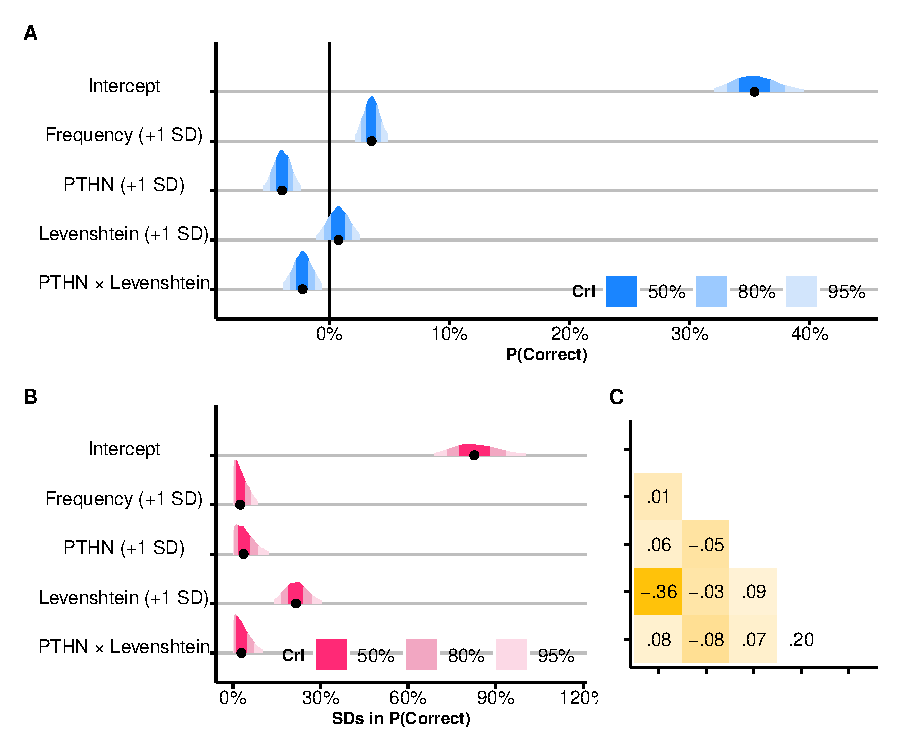
\includegraphics{manuscript_files/figure-latex/posteriorfix-1.pdf}
\caption{\label{fig:posteriorfix}Estimated posterior distributions of coefficients in Model 3. A) Population-level effects. Distributions indicate the estimated posterior likelihood density of each coefficient. Credible intervals \(CrI\), represented with increasingly lighter segmentents in the distribution indicate the range of values that contain the true value with 95\%, 80\%, and 50\% probability. Dots represent the mean of the distribution. B) Participant-level coefficient variability. Our model estimated participant-level coefficients to account for the dependency between responses from the same participant. Distributions in this panel indicate the estimated variability across coefficients from different participants, expressed as standard deviations \(SD\). C) Correlation between participant-level effects. Our model allowed participant-level coefficients to co-vary. This panel represents the Pearson correlations between each pair of coefficients, expressed as the mean of the posterior distribution of each correlation. Coefficients are represented in the X-axis and Y-axis in the same order as indicated in the Y-axis of panels A and C.}
\end{figure}

Overall, participants were 35.45\%, (\emph{SE} = 52.06\%, 95\% \emph{CrI} = {[}32.09\%, 39.47\%{]}) likely to produce correct translations. Every standard deviation increment in the translation's lexical frequency (\emph{SD} = 0.59) increased the probability of a correct responses in 3.53\% (\emph{SE} = 0.67\%, 95\% \emph{CrI} = {[}2.21\%, 4.85\%{]}). The number of the translation's more frequent phonological neighbours, on the other hand, decreased the probability of a correct responses in -3.90\% (\emph{SE} = 0.76\%, 95\% \emph{CrI} = {[}-5.42\%, -2.43\%{]}) for every increase in 1 \emph{SD} (3.65). The effect of phonological similarity was conditional to the phonological density of the translation. Phonological similarity barely increased the probability of a correct responses (0.78\%, \emph{SE} = 1\%, 95\% \emph{CrI} = {[}-1.02\%, 3\%{]}) by itself. However, for every \emph{SD} increase in PTHN, phonological similarity increased in -2\%, (\emph{SE} = 0.80\%, 95\% \emph{CrI} = {[}-3.78\%, -0.68\%{]}) such probability.

\begin{figure}
\centering
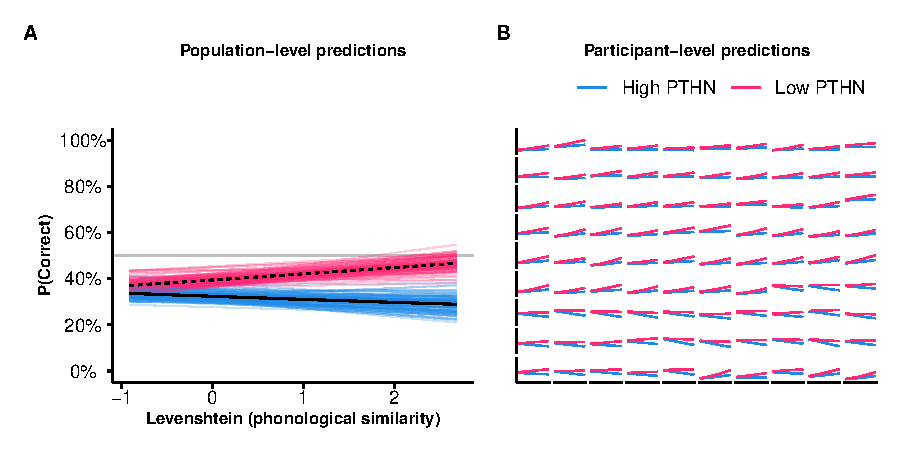
\includegraphics{manuscript_files/figure-latex/marginaleffects-1.pdf}
\caption{\label{fig:marginaleffects}Expected mean posterior predictions. A) Population-level expected mean posterior predictions. The X-axis and the Y-axis represent the Levenshtein distance (in standard deviations from the mean) and the probability of correct translation, respectively. We simulated 200 observations from our model: 100 simulations for words with low PTHN (-1 SD) and 100 simulations for high PTHN (+1 SD) words. We did this across the range of values of the Levenshtein scores. For each simulation, we drew a single sample from the posterior distribution of each coefficient. Each simulation is depicted in the graph as a line: pink in the case of low PTHN words, and blue in the case of high PTHN words. We also plotted the mean of the high PTHN (black solid line) and low PTHN (black dashed line) simulations to indicate the expected mean value of the posterior predictions of the model. The dispersion of the lines indicates the uncertainty of our predictions. B) Participant-level expected mean posterior predictions. We conducted the same procedure for each individual participant, simulating 100 observations for high-PTHN and 100 for low-PTHN from our model acrosss the range of Levenshtein scores. We averaged the resulting predictions for each participant and then plotted each participant's predictions in separate panels to show how the effect of PTHN and phonological similarity changed at the individual level.}
\end{figure}

\hypertarget{discussion}{%
\section{Discussion}\label{discussion}}

\newpage

\hypertarget{references}{%
\section{References}\label{references}}

\begingroup
\setlength{\parindent}{-0.5in}
\setlength{\leftskip}{0.5in}

\hypertarget{refs}{}
\begin{CSLReferences}{1}{0}
\leavevmode\vadjust pre{\hypertarget{ref-boada2020subtlex}{}}%
Boada, R., Guasch, M., Haro, J., Demestre, J., \& Ferré, P. (2020). SUBTLEX-CAT: Subtitle word frequencies and contextual diversity for catalan. \emph{Behavior Research Methods}, \emph{52}(1), 360--375.

\leavevmode\vadjust pre{\hypertarget{ref-broersma2021praat}{}}%
Broersma, P., \& Weenink, D. (2021). Praat: Doing phonetics by computer {[}computer program{]} (Version Version 6.1.54). Retrieved from \url{http://www.praat.org/}

\leavevmode\vadjust pre{\hypertarget{ref-burkner2017brms}{}}%
Bürkner, P.-C. (2017). Brms: An r package for bayesian multilevel models using stan. \emph{Journal of Statistical Software}, \emph{80}(1), 1--28.

\leavevmode\vadjust pre{\hypertarget{ref-carpenter2017stan}{}}%
Carpenter, B., Gelman, A., Hoffman, M. D., Lee, D., Goodrich, B., Betancourt, M., \ldots{} Riddell, A. (2017). Stan: A probabilistic programming language. \emph{Grantee Submission}, \emph{76}(1), 1--32.

\leavevmode\vadjust pre{\hypertarget{ref-christoffels2006memory}{}}%
Christoffels, I. K., De Groot, A. M., \& Kroll, J. F. (2006). Memory and language skills in simultaneous interpreters: The role of expertise and language proficiency. \emph{Journal of Memory and Language}, \emph{54}(3), 324--345.

\leavevmode\vadjust pre{\hypertarget{ref-christoffels2013language}{}}%
Christoffels, I. K., Ganushchak, L., \& Koester, D. (2013). Language conflict in translation: An ERP study of translation production. \emph{Journal of Cognitive Psychology}, \emph{25}(5), 646--664.

\leavevmode\vadjust pre{\hypertarget{ref-collins1975spreading}{}}%
Collins, A. M., \& Loftus, E. F. (1975). A spreading-activation theory of semantic processing. \emph{Psychological Review}, \emph{82}(6), 407.

\leavevmode\vadjust pre{\hypertarget{ref-costa2000cognate}{}}%
Costa, A., Caramazza, A., \& Sebastian-Galles, N. (2000). The cognate facilitation effect: Implications for models of lexical access. \emph{Journal of Experimental Psychology: Learning, Memory, and Cognition}, \emph{26}(5), 1283.

\leavevmode\vadjust pre{\hypertarget{ref-cuetos2011subtlex}{}}%
Cuetos, F., Glez-Nosti, M., Barbon, A., \& Brysbaert, M. (2011). SUBTLEX-ESP: Frecuencias de las palabras espanolas basadas en los subtitulos de las peliculas. \emph{Psicol{ó}gica}, \emph{32}(2), 133--144.

\leavevmode\vadjust pre{\hypertarget{ref-de2000hard}{}}%
De Groot, A. M., \& Keijzer, R. (2000). What is hard to learn is easy to forget: The roles of word concreteness, cognate status, and word frequency in foreign-language vocabulary learning and forgetting. \emph{Language Learning}, \emph{50}(1), 1--56.

\leavevmode\vadjust pre{\hypertarget{ref-de1982relationship}{}}%
De Haan, H. J. (1982). The relationship of estimated comprehensibility to the rate of connected speech. \emph{Perception \& Psychophysics}, \emph{32}(1), 27--31.

\leavevmode\vadjust pre{\hypertarget{ref-degroot1994forward}{}}%
Degroot, A. M., Dannenburg, L., \& Vanhell, J. G. (1994). Forward and backward word translation by bilinguals. \emph{Journal of Memory and Language}, \emph{33}(5), 600--629.

\leavevmode\vadjust pre{\hypertarget{ref-dijkstra2019multilink}{}}%
Dijkstra, T., Wahl, A., Buytenhuijs, F., Van Halem, N., Al-Jibouri, Z., De Korte, M., \& Rekké, S. (2019). Multilink: A computational model for bilingual word recognition and word translation. \emph{Bilingualism: Language and Cognition}, \emph{22}(4), 657--679.

\leavevmode\vadjust pre{\hypertarget{ref-gelman2020regression}{}}%
Gelman, A., Hill, J., \& Vehtari, A. (2020). \emph{Regression and other stories}. Cambridge University Press.

\leavevmode\vadjust pre{\hypertarget{ref-goldinger1989priming}{}}%
Goldinger, S. D., Luce, P. A., \& Pisoni, D. B. (1989). Priming lexical neighbors of spoken words: Effects of competition and inhibition. \emph{Journal of Memory and Language}, \emph{28}(5), 501--518.

\leavevmode\vadjust pre{\hypertarget{ref-de1992determinants}{}}%
Groot, A. M. de. (1992). Determinants of word translation. \emph{Journal of Experimental Psychology: Learning, Memory, and Cognition}, \emph{18}(5), 1001.

\leavevmode\vadjust pre{\hypertarget{ref-kroll1994category}{}}%
Kroll, J. F., \& Stewart, E. (1994). Category interference in translation and picture naming: Evidence for asymmetric connections between bilingual memory representations. \emph{Journal of Memory and Language}, \emph{33}(2), 149--174.

\leavevmode\vadjust pre{\hypertarget{ref-levenshtein1966binary}{}}%
Levenshtein, V. I., \& others. (1966). Binary codes capable of correcting deletions, insertions, and reversals. In \emph{Soviet physics doklady} (Vol. 10, pp. 707--710). Soviet Union.

\leavevmode\vadjust pre{\hypertarget{ref-lotto1998effects}{}}%
Lotto, L., \& De Groot, A. M. (1998). Effects of learning method and word type on acquiring vocabulary in an unfamiliar language. \emph{Language Learning}, \emph{48}(1), 31--69.

\leavevmode\vadjust pre{\hypertarget{ref-luce1998recognizing}{}}%
Luce, P. A., \& Pisoni, D. B. (1998). Recognizing spoken words: The neighborhood activation model. \emph{Ear and Hearing}, \emph{19}(1), 1.

\leavevmode\vadjust pre{\hypertarget{ref-luce1990similarity}{}}%
Luce, P. A., Pisoni, D. B., \& Goldinger, S. D. (1990). Similarity neighborhoods of spoken words.

\leavevmode\vadjust pre{\hypertarget{ref-marian2012clearpond}{}}%
Marian, V., Bartolotti, J., Chabal, S., \& Shook, A. (2012). CLEARPOND: Cross-linguistic easy-access resource for phonological and orthographic neighborhood densities.

\leavevmode\vadjust pre{\hypertarget{ref-mcclelland1981interactive}{}}%
McClelland, J. L., \& Rumelhart, D. E. (1981). An interactive activation model of context effects in letter perception: I. An account of basic findings. \emph{Psychological Review}, \emph{88}(5), 375.

\leavevmode\vadjust pre{\hypertarget{ref-peirce2019psychopy2}{}}%
Peirce, J., Gray, J. R., Simpson, S., MacAskill, M., Höchenberger, R., Sogo, H., \ldots{} Lindeløv, J. K. (2019). PsychoPy2: Experiments in behavior made easy. \emph{Behavior Research Methods}, \emph{51}(1), 195--203.

\leavevmode\vadjust pre{\hypertarget{ref-potter1984lexical}{}}%
Potter, M. C., So, K.-F., Von Eckardt, B., \& Feldman, L. B. (1984). Lexical and conceptual representation in beginning and proficient bilinguals. \emph{Journal of Verbal Learning and Verbal Behavior}, \emph{23}(1), 23--38.

\leavevmode\vadjust pre{\hypertarget{ref-rcore2019r}{}}%
RCore, T. (2019). R: A language and environment for statistical computing. R foundation for statistical computing, austria.

\leavevmode\vadjust pre{\hypertarget{ref-schepens2012distributions}{}}%
Schepens, J., Dijkstra, T., \& Grootjen, F. (2012). Distributions of cognates in europe as based on levenshtein distance. \emph{Bilingualism: Language and Cognition}, \emph{15}(1), 157--166.

\leavevmode\vadjust pre{\hypertarget{ref-thierry2007brain}{}}%
Thierry, G., \& Wu, Y. J. (2007). Brain potentials reveal unconscious translation during foreign-language comprehension. \emph{Proceedings of the National Academy of Sciences}, \emph{104}(30), 12530--12535.

\leavevmode\vadjust pre{\hypertarget{ref-van2014stringdist}{}}%
van der Loo, M. P. J. (2014). The stringdist package for approximate string matching. \emph{The {R} {J}ournal}, \emph{6}, 111--122. Retrieved from \url{https://CRAN.R-project.org/package=stringdist}

\leavevmode\vadjust pre{\hypertarget{ref-van1998orthographic}{}}%
Van Heuven, W. J., Dijkstra, T., \& Grainger, J. (1998). Orthographic neighborhood effects in bilingual word recognition. \emph{Journal of Memory and Language}, \emph{39}(3), 458--483.

\leavevmode\vadjust pre{\hypertarget{ref-van2014subtlex}{}}%
Van Heuven, W. J., Mandera, P., Keuleers, E., \& Brysbaert, M. (2014). SUBTLEX-UK: A new and improved word frequency database for british english. \emph{Quarterly Journal of Experimental Psychology}, \emph{67}(6), 1176--1190.

\leavevmode\vadjust pre{\hypertarget{ref-vehtari2017practical}{}}%
Vehtari, A., Gelman, A., \& Gabry, J. (2017). Practical bayesian model evaluation using leave-one-out cross-validation and WAIC. \emph{Statistics and Computing}, \emph{27}(5), 1413--1432.

\leavevmode\vadjust pre{\hypertarget{ref-warren1970perceptual}{}}%
Warren, R. M. (1970). Perceptual restoration of missing speech sounds. \emph{Science}, \emph{167}(3917), 392--393.

\end{CSLReferences}

\endgroup

\newpage

\hypertarget{appendix}{%
\section{Appendix}\label{appendix}}

\begin{figure}
\centering
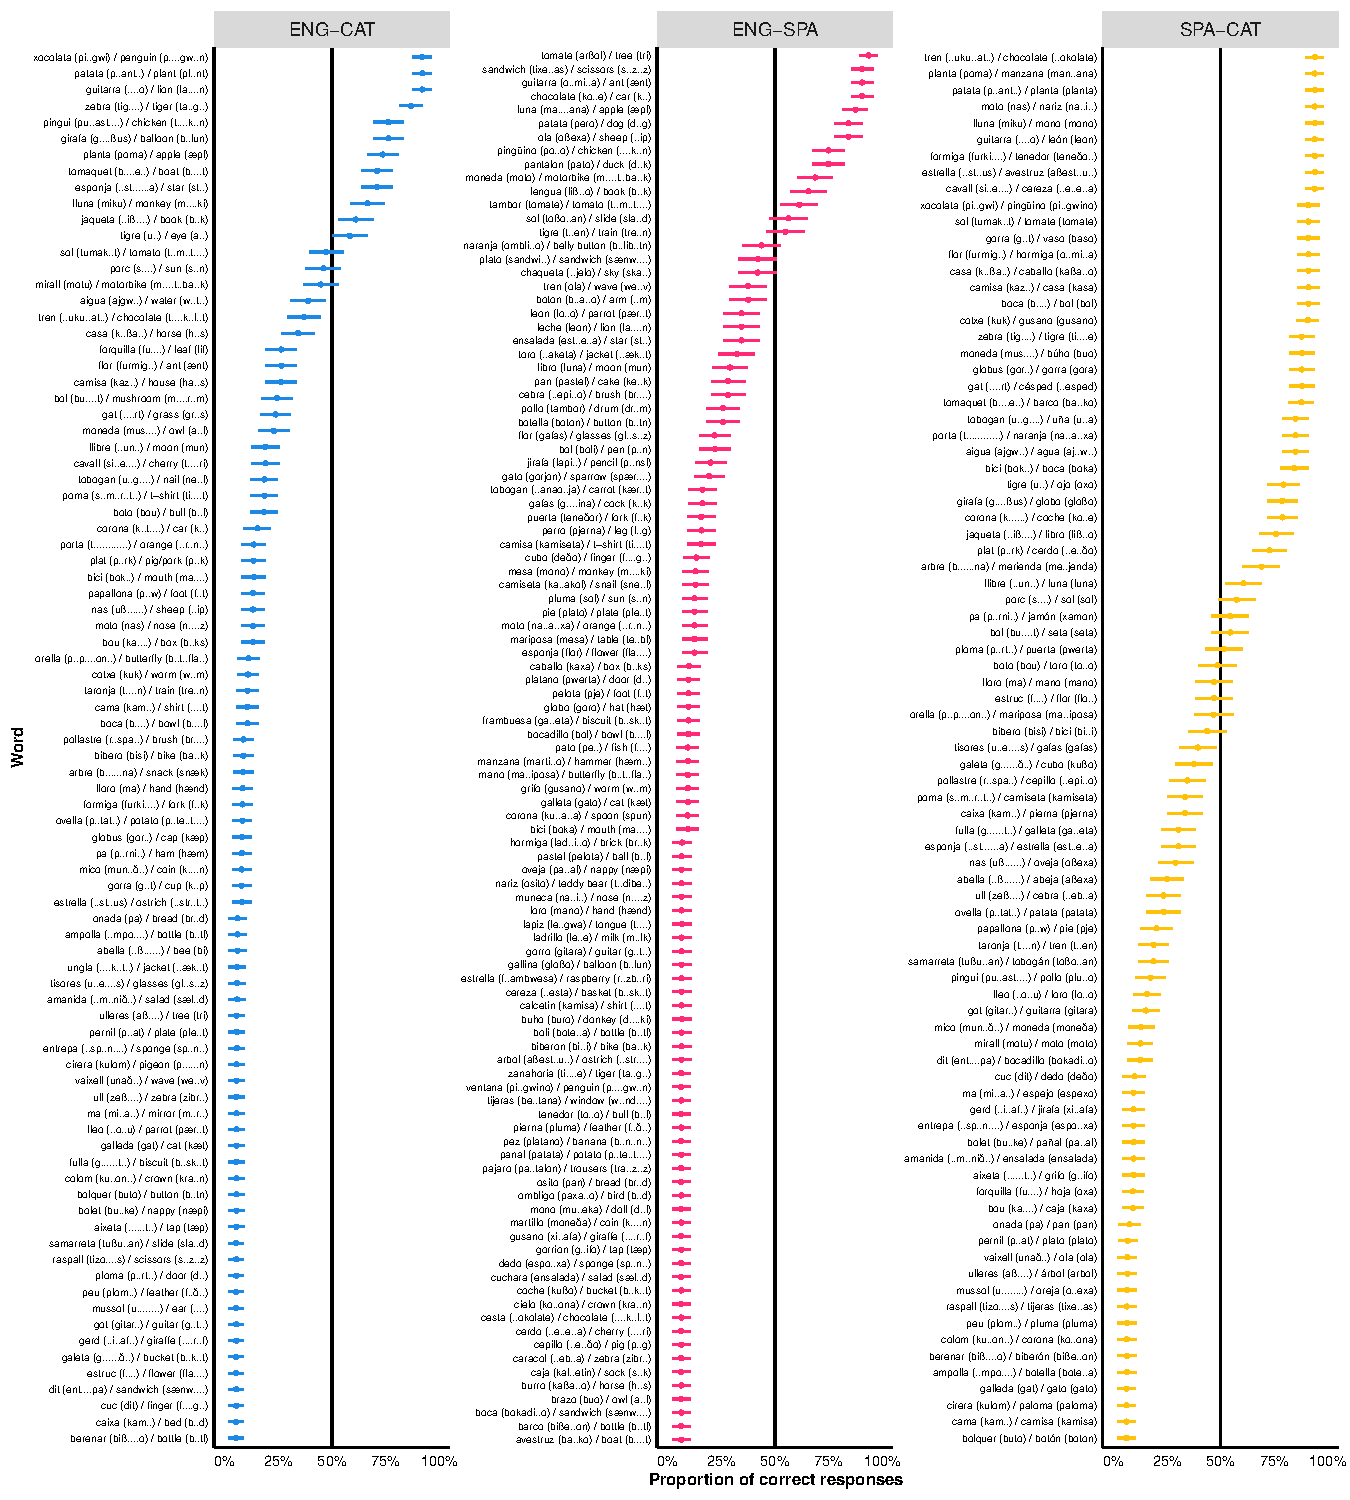
\includegraphics{manuscript_files/figure-latex/accuracy-1.pdf}
\caption{\label{fig:accuracy}Proportion of correct translation by item. Words presented to participants in the English-Spanish or in the English-Catalan and Spanish-Catalan are listed in the Y-axis, ordered from higher to lower average translation accuracy, depicted in the X-axis. Dots and whiskers represent the average accuracy and 95\% confidence interval of each word. Accuracy is plotted separately for each group.}
\end{figure}


\end{document}
